\chapter{Mathematica Modelling of Wheeled Mobile Platform }
\label{c4_SenCal}
In the field of mobile robotics extensive research has been carried out. Mobile robots can broadly be divided into three categorises-wheeled robots, legged robots ~\cite{machado2006overview} and aerial vehicles ~\cite{valavanis2014handbook}. There are few mobile robots which uses both wheels and legs for locomotion for example the Creadapt  \cite{mouret2015evolutionary}, in order to take advantage of both modes of locomotion. Among these the most extensively studied are the  Wheeled mobile robots (WMR). They have been classified in to five generic classes by Champion et.al \cite{campion1996structural},~\cite{campion2008wheeled}  based on there mobility resulting from the kinematic constrains due to  different wheel types. The most common among these are the  3 wheeled differential driven WMR with one castor wheels. Because of its simplicity in modelling, they have been used in most of the  control and motion planing algorithm  \cite{desantis1995modeling}, \cite{koh1999smooth} and \cite{d1995control}. 

In order to develop a model based control algorithm it is imperative to have good dynamic model of the WMR. These dynamic models are used in  simulation software,  Software in Loop (SIL) testing and Hardware in Loop testing of controllers.   Different methods has been adopted to derive the dynamic model of WMR. A general dynamical model is derived for three-wheel mobile robots with nonholonomic constraints by using a Lagrange formulation by B. d'Andrea-Novel \cite{d1991modelling}.  Where as Thanjavur and Rajagopalan \cite{thanjavur1997ease} has used Kane's method  and  Saha et. al. \cite{saha1991dynamics},\cite{saha1989kinematics} uses natural orthogonal compliment (NOC) method.  
 
All the papers known to us uses, the standard caster wheel in deriving the dynamic model of the WMR. In this paper we have presented the modelling of Castor wheel in the most general configuration. In the stranded castor wheel the axis of rotation is perpendicular to the line joining the pivot and the axis of rotation as shown in Figure \ref{fig:std}. Where as in our case they oriented in  the most general way as shown in figure Figure \ref{fig:gen}. We have used the Natural Orthogonal Compliment approach as it inherently takes care of the non-holonomic constraint of the wheels. Moreover being a matrix based approach it is convenient for numerical simulations. The paper is divide in to three parts in the first part we briefly introduce the concept of NOC method, in the second part the derivation of dynamic model of WMR is presented, in the last part we discuss few special cases which can be derived from our model.
\section{Natural Orthogonal Compliment (NOC) Method}
Let us consider a system $n$ rigid body, interconnected with different types of joints. Let, $f_i$ be the net force acting at the center of mass (CM) of the $i-th$  body and $n_i$ is the net moment. If $m_i$ is the mass, $I_{ci}$ moment of inertia with respect to  CM, $c_i$ position vector of CM and $\omega_i$ the angular velocity of the same body. Then equation of motion of $i-th$ rigid body is given by Newton-Euler equations \ref{NE}. 
\begin{equation}
\label{NE}
f_i=m_i\ddot{c_i} \quad and \quad n_i=I_{ci} \omega_i+\omega_i \times I_{ci} \omega_i
\end{equation}
If we define, twist ($t$) and wrench($w$) as 
\begin{equation*}
t_i=\begin{pmatrix}
\omega_i\\ \dot{c_i}
\end{pmatrix} \quad
w_i=\begin{pmatrix}
n_i\\f_i
\end{pmatrix}
\end{equation*}
The wrench $w_i$ acting on the $i-th$ body can be decomposed into $w^w_i$, called the \textit{working component} and  $w^C_i$, the \textit{non-working component}. The working component consists if all the forces and torques, which imparts/extracts energy to/from the system, i.e. motor actuating torque. The non-working component of the wrench consists of the forces and torques which are used to constrain the motion of the body at the joints.
Then Newton-Euler Equation (\ref{NE}) can be rewritten  in a single matrix equation as 
\begin{equation}
\label{2}
M_i\dot{t_i}+W_iM_it_i=w^w_i+w^c_i \quad \because w_i=w^w_i+w^c_i
\end{equation}
\begin{equation}
\label{3}
M_i=\begin{pmatrix}
I_{ci} & 0\\0 & m_i\tilde{1}
\end{pmatrix} ,
\quad W_i=\begin{pmatrix}
\Omega_i &0\\0&0
\end{pmatrix},
\quad
\Omega_i=\omega_i\times \tilde{1}
\end{equation}
Where $\omega_i\times 1$, is refered as the cross product matrix of vector $\omega_i$ and $\tilde{1}$, denotes the identity matrix, for details refer to \cite{angeles2013fundamentals},\cite{saha2010robotics}.
The equation of all the $n$ rigid body in the system can be collected and written as a single matrix equation (\ref{DCE}) referred to as  decoupled equation of motion of the system. 
\begin{equation}
\label{DCE}
M\dot{t}+WMt=w^c+w^w
\end{equation}
Where
\[M=diag[M_1,M_2,...M_n[, \quad W=diag[W_1,W_2,...W_n], \quad t=[t_1^T,t_2^T, ....t_n^T]^T\]
\[ w^j=[{w_1^j}^T,{w_2^j}^T, ....{w_n^j}^T]^T, \,j=c,w \]

The kinematic constraint both holonomic and non-holonomic (i.e. pure rolling) between two bodies $i$ and $j$ of a system, give rise to linear homogeneous system of algebraic equations \cite{angeles2013fundamentals} as given below, where $A_i,A_j$ depend on the DH parameters.
\begin{equation}
A_it_i+A_jt_j=0
\end{equation}
The constraint equations corresponding to all the joints in the system can be written in terms of the \textit{generalized twist vector} $t$. Furthermore if, $ \dot{\theta}=(\dot{\theta_1},\dot{\theta_2},....)$ denote the \textit{independent generalized velocity} of the system, we can then write $t$ in terms of $\dot{\theta}$ as $t=T\dot{\theta}$. Using the fact, that $\dot{\theta}$ can take any arbitrary value, we get
\begin{equation}
\label{AT}
At=0 , \quad \Rightarrow  AT\dot{\theta}=0\quad \Rightarrow AT=0
\end{equation}
The above equation (\ref{AT}) indicates that $T$ is the orthogonal compliment of $A$. Since this relation arises naturally, hence the name \textit{Natural Orthogonal Compliment}. It can be shown \cite{angeles2013fundamentals} that the non-working wrench $w^c$, lies in the range space of $A^T$. In view of equation \ref{AT}, it can be proved that $w^c$ lies in the null space of $T^T$, therefore
\begin{equation}
T^Tw^c=0
\end{equation}
To eliminate the non-working forces and moments, i.e $w^C$ from the uncoupled equation of motion (\ref{DCE}), we multiply both sides of equation \ref{DCE} by $T^T$.
\begin{equation}
 T^TM\dot{t}+T^TWMt=T^Tw^W, \quad
 \Rightarrow T^TMT\ddot{\theta}+T^T(M\dot{T}+WMT)\dot{\theta}=T^Tw^T
\end{equation}
Equation \ref{CE} represents the dynamic equation of  interconnected $n$-body system. This equation can be expressed in terms of the independent generalized velocity $\dot{\theta}$ and generalized acceleration $\ddot{\theta}$, by using the relations $t=T\dot{\theta}$ and $\dot{t}=\dot{T}\dot{\theta}+T\ddot{\theta}$  in equation \ref{CE}.
thus the final equations of motion can be written as

\begin{equation}
\label{CE}
or\quad \quad I(\theta)\ddot{\theta}=C(\theta,\dot{\theta})\dot{\theta}+\tau
\end{equation}
Where
\[I(\theta)\equiv T^TMT,\text{generalized inertia matrix}\]
\[C(\theta,\dot{\theta})\equiv -T^T(M\dot{T}+WMT)\dot{\theta}, \text{convective inertia matrix}\]
\[\tau\equiv T^Tw^T,\text{ generalized driving force vectcor}\]


\begin{figure}
	\begin{minipage}[t]{0.5\textwidth}
	\centering
		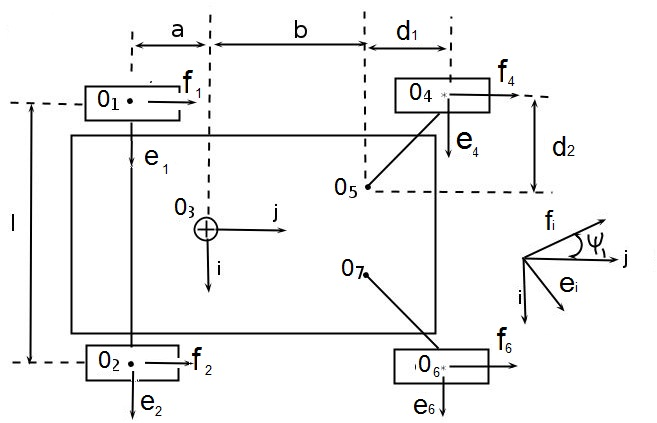
\includegraphics[width=3.5in]{Chapter4/fig/fig2.jpg} 
		\caption{WMR-general}\label{fig:gen}
	\end{minipage}
	\hfill
	\begin{minipage}[t]{0.5\textwidth}
	\centering
		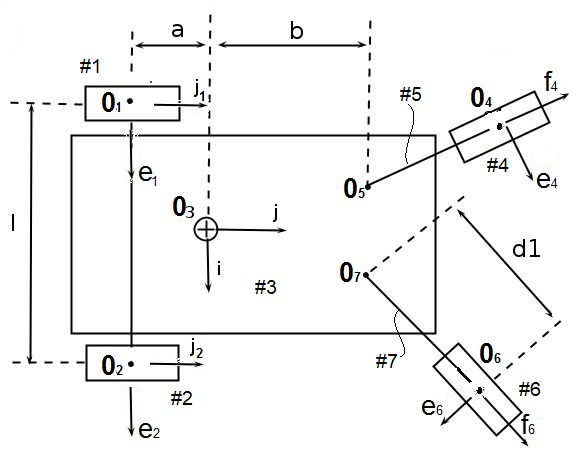
\includegraphics[width=3in]{Chapter4/fig/fig1.jpg} 
		\caption{WMR-Std. Castor}\label{fig:std}
	\end{minipage}
\caption{Castor wheel Configuration of WMR}
\end{figure}


\section{Dynamic Equation of WMR}
The dynamic equation of a differentially driven 3 wheeled mobile platform based on Natural orthogonal compliment metohod has been presented by Saha\cite{saha1991dynamics}. The vehicle consisted of 2 driven wheel and one standard caster wheel.In general for large vehicles it necessary to have at least four wheels, for the point of stability of the vehicle.Such a vehicle is shown in figure 1. It may be noted that the caster wheels used in this case are the standered caster wheel configuration, where the angle between line $O_4O_3$ and vector $e_3$ is  $90\deg$. This is a special case of the more general configuration of the caster wheel which are shown in figure 2, where angle between line $O_4O_3$ and vector $e_3$ is not $90\deg$

 The vehicle we have considered in this paper is shown in figure 2. It consist two independently driven wheels at the back and two generalized caster wheels at the front. The actuated wheels are labelled as body \#1 and \#2. The platform is body \#3, The first caster wheel and its bracket is labelled as \#4 and \#5, with the castor pivoted at $O_4$. Similarly the second castor is pivoted at $O_6$, and its bracket and wheel is labelled as \#6 an \#7. All the wheels are assumed to be rolling with out slipping.  
\subsection{Kinematic analysis}
In order to proceed with the kinematic analysis of the vehicle in figure 1, we define a orthogonal triad of vectors ${i,j,k}$ at point $O_3$, the control point of the platform, as shown in the figure. If $\dot{\theta_1}$ and $\dot{\theta_2}$ denotes the rate of rotation of wheel \#1 and \#2. Then the linear velocity of point $O_1\&O_2$ under pure rolling condition is given by 
\begin{equation}
\label{velO1}
\dot{O_i}=r\dot{\theta_j}, \quad \text{r=radius of wheel}
\end{equation}
The angular velocity of the platform $\omega_3$ can be written as 
\begin{equation}
\label{omegaPlat}
\omega_3=(r/l)(\dot{\theta_1}-\dot{\theta_2}).
\end{equation}
Further, the velocity of point $o_3$ can be written as
$\dot{o_3}=\dot{o_i}+\omega_3 \times (c-o_i), \quad i=1,2$. where, $o_3 $ and $o_i$  is the position vector of point $O_3$ and $O_i$ respectively, with respect to some  point fixed to the ground. By eliminate $\omega_3$ from  these two equation, we get
\begin{equation}
\label{velPlat}
 \quad \quad \dot{o_3}=(ar/l)(\dot{\theta_1}-\dot{\theta_2})+(r/2)(\dot{\theta_1}+\dot{\theta_2})
\end{equation}

Now, the the angular velocity of the drive wheel \#1 can be expressed as $\omega_1=-\dot{\theta_1}i+\omega_3k$, using equation \ref{omegaPlat}, we can write 
\begin{equation}
\label{omegaWheel1}
\omega_1=\begin{pmatrix}
-i+(r/l)k & -(r/l)k
\end{pmatrix}
\begin{pmatrix}
\dot{\theta_1}\\\dot{\theta_2}
\end{pmatrix}
\end{equation}
Using equation \ref{velO1} and \ref{omegaWheel1}, we can write the twist for wheel \#1 in terms of $\dot{\theta_a}$, as 
\begin{equation}
\label{twist1}
t_1=\begin{pmatrix}
\omega_1\\\dot{o_1}
\end{pmatrix}=
\begin{pmatrix}
-i+(r/l)k & -(r/l)k\\ rj & 0
\end{pmatrix}
\begin{pmatrix}
\dot{\theta_1}\\\dot{\theta_2}
\end{pmatrix}
\end{equation}

Similarly, for the other actuated wheel \#2, we get

\begin{equation}
\label{twist2}
t_2=\begin{pmatrix}
\omega_1\\\dot{o_1}
\end{pmatrix}=
\begin{pmatrix}
-i+(r/l)k & -(r/l)k\\  0 &rj
\end{pmatrix}
\begin{pmatrix}
\dot{\theta_1}\\\dot{\theta_2}
\end{pmatrix}
\end{equation}
To calculate the twist, $t_3$ of the platform, body \#3, we use combine equation \ref{omegaPlat} and \ref{velPlat}, and get
\begin{equation}
\label{twist3}
t_3=\begin{pmatrix}
\omega_3\\\dot{o_3}
\end{pmatrix}=
\begin{pmatrix}
\rho\delta & -\rho\delta\\
r(\lambda i+(1/2)j & r(-\lambda i+(1/2)j
\end{pmatrix}
\begin{pmatrix}
\dot{\theta_1}\\\dot{\theta_2}
\end{pmatrix}
\end{equation}
where
\[ \delta\equiv d/l, \quad \rho \equiv r/d, \quad \lambda \equiv a/l \]
In order to calculate the twist of the caster bracket and the caster wheel, we need to express the  unactuated joint rates $\dot{\psi_1}$ and $\dot{\phi_1}$, in terms of actuated angle rate vector $\dot{\theta_a}$. Where, $\dot{\psi_1}$ denotes the rate of rotation of bracket, body \#5 about $O_4$ with respect to the platform, and 
$\dot{\phi_1}$ the rate of rotation of caster wheel, body \#4 about its axis $e_3$, with respect to bracket. The velocity of $O_5$ can be expressed in two independent forms, one in terms of the velocity of $o_3$ and the other in terms of the velocity of $o_5$, i.e
\begin{equation}
\dot{o_5}=\dot{o_4}+\omega_5\times(d_1e_4-d2f_4), \quad
\dot{o_5}=\dot{o_4}+\omega_5\times(d_1e_4-d2f_4)
\end{equation}
On equating the above to equations together, and using the rotation matrix between coordiante system $\{i,j,k\}$ and $\{e_4,f_4,k\}$, to express the equation in $e_4\&f_4$, we get
\begin{equation}
(-\dot{\phi_1}r+\dot{\psi_1}d_1)f_3+d_3\dot{\psi_1}e_3=\dot{o_3}
+\omega_3(m\cos\psi_1-b\sin\psi_1-d_1)e_4
\end{equation} 
Taking the dot product of the above equation first with $e_4$ and then with $f_4$, and using equation \ref{velPlat} for $\dot{o_3}$, we get
\begin{equation}
\label{unac2act1}
\begin{pmatrix}
d_2&0\\-d_1 &r
\end{pmatrix}
\begin{pmatrix}
\dot{\psi_1}\\ \dot{\phi_1}
\end{pmatrix}
=\begin{pmatrix}
(-ar/l)S_{\psi_1}+(r/2)C_{\psi_1}+\delta_1 & 
(ar/l)S_{\psi_1}+(r/2)C_{\psi_1}-\delta_1 \\
(ar/l)C_{\psi_1}+(r/2)S_{\psi_1}+\delta_2 & 
(-ar/l)C_{\psi_1}+(r/2)S_{\psi_1}-\delta_2 
\end{pmatrix}\dot{\theta_a}=[F_{ij}]\dot{\theta_a}
\end{equation}
where, 
\[ \delta_1=(r/l)(mC_{\psi_1}-bS_{\psi_1}-d2, \quad  \delta_2=(r/l)(mS_{\psi_1}+bC_{\psi_1}+d1 \]

Similarly for the other caster wheel we get,
\begin{equation}
\label{unac2act2}
\begin{pmatrix}
d_2&0\\-d_1 &r
\end{pmatrix}
\begin{pmatrix}
\dot{\psi_2}\\ \dot{\phi_2}
\end{pmatrix}
=\begin{pmatrix}
(-ar/l)S_{\psi_2}+(r/2)C_{\psi_2}-\delta_3 & 
(ar/l)S_{\psi_2}+(r/2)C_{\psi_2}+\delta_3 \\
(ar/l)C_{\psi_2}+(r/2)S_{\psi_2}+\delta_4 & 
(-ar/l)C_{\psi_2}+(r/2)S_{\psi_2}-\delta_4 
\end{pmatrix}\dot{\theta_a}=[G_{ij}]\dot{\theta_a}
\end{equation}
where, 
\[ \delta_3=(r/l)(mC_{\psi_2}+bS_{\psi_2}+d2, \quad  \delta_4=(r/l)(mS_{\psi_2}+bC_{\psi_2}+d1 \]




 The angular and the liner velocity of the c.g.of the caster wheel,\#4 is  written in-terms of the co-ordinate frame fixed to the bracket \#5, $\{e_4,f_4,k\}$, as
\begin{equation}
\label{omegacastor1}
\omega_4=\dot{\phi_1}e_4+(\omega_3+\dot{\psi_1})k, \quad
\dot{o_4}=\dot{\phi_1}e_4
\end{equation}
Using equation \ref{unac2act1} and \ref{omegaPlat}, the twist $t_4$ can be written as
\begin{equation}
\label{twist4}
t_4=\begin{pmatrix}
\Theta_4\\C_4
\end{pmatrix}\dot{\theta_a}
\end{equation}
where
\[ \Theta_4=[F_{11}e_4+\bar{F_{21}}k \quad F_{12}e_4+\bar{F_{22}}k],\quad 
C_4=r[-F_{11}f_4 \quad -F_{12}f_4]\]
\[\bar{F_{21}}=F_{21}+\rho \delta, \quad \bar{F_{22}}=F_{22}-\rho\delta\]

The angular and the liner velocity of the c.g.of the caster bracket,\#5 is  written in-terms of the co-ordinate frame fixed to the bracket, as
\begin{equation}
\omega_4=\dot{\phi_1}e_3+\dot{\psi_1}k, \quad
\dot{o_4}=\dot{o_4}+\omega_5\times [-df_3]
\end{equation}
Now using equations\ref{unac2act1}\& \ref{omegaPlat}, the twist $t_5$ can be written as
\begin{equation}
\label{twist5}
t_5=\begin{pmatrix}
\Theta_5\\C_5
\end{pmatrix}\dot{\theta_a}
\end{equation}
where
\[ \Theta_5=[\bar{F_{21}}k \quad \bar{F_{22}}k],\quad 
C_5=d[(1/2)bar{F_{21}}e_4-\rho F_{11}f_4 \quad (1/2)bar{F_{22}}e_4-\rho F_{12}f_4]\]
In similar manner the twist $t_6 \& t_7$  of the other caster wheel and its bracket can be written as 
\begin{equation}
\label{twist6}
t_6=\begin{pmatrix}
\Theta_6\\C_6
\end{pmatrix}\dot{\theta_a}, \quad t_7=\begin{pmatrix}
\Theta_7\\C7
\end{pmatrix}\dot{\theta_a}
\end{equation}
where
\[ \Theta_6=[G_{11}e_6+\bar{G_{21}}k \quad G_{12}e_6+\bar{G_{22}}k],\quad 
C_6=r[-G_{11}f_6 \quad -G_{12}f_6]\]
\[ \Theta_7=[\bar{G_{21}}k \quad \bar{G_{22}}k],\quad 
C_7=d[(1/2)bar{G_{21}}e_6-\rho G_{11}f_6 \quad (1/2)bar{G_{22}}e_6-\rho G_{12}f_6]\]
\[\bar{G_{21}}=G_{21}+\rho \delta, \quad \bar{G_{22}}=G_{22}-\rho\delta\] 

\subsection*{Dynamic Equations}
Based on the twist calculated in terms of the independent actuation vector $\dot{\theta_a}$, we now derive the generalized inertia matrix and the Convective inertia term for the coupled equation of motion \ref{CE}.
\subsubsection*{Generalized Inertia Matrix, $I$}
 From the above equations of twist of individual body we get  $t_i=T_i\dot{\theta_a}$, by definition  $t=[t_1^T, t_2^T....t_7^T]^T$. Therefore, we get  \[T=[T_1^T, T_2^T,... T_7]^T\]. Since the matrix $M$ is block diagonal
\begin{equation}
I=T^TMT=T_1^TM_1T_1+T_2^TM_2T_2+...T_7^TM_7T_7
\end{equation}
\begin{equation}
I_m=\sum_{i=1,2}T_i^TM_iT_i=\begin{pmatrix}
I_w+(\rho\delta)^2H++m_wr^2 & -2(\rho\delta)^2H
\\
-2(\rho\delta)^2H &I+(\rho\delta)^2H++m_wr^2
\end{pmatrix} \quad \mathtt{ where} M_i=\begin{pmatrix}
I_w &0\\0 & m_w\mathbf{1}
\end{pmatrix}
\end{equation}
Where $\tilde{I_w}=\begin{pmatrix}
I_w&0&0\\0&H&\\0&0&H
\end{pmatrix}$ is the $3\times 3$ moment of Inertia matrix expressed in co-ordinate $\{i,j,i\}$, $m_w$ is the mass of the motorized wheels, and $1$ is$3\times 3$ identity matrix.
\\
If the mass of the platform is $m_p$ and its moment of inertia about vector $\mathbf{k}$ is $I_p$, then \cite{angeles2013fundamentals} 
\begin{equation}
I_3=T^T_3M_3T_3=I_p(\rho\delta)^2\begin{pmatrix}
1&-1\\-1&1
\end{pmatrix}
+m_pr^2\begin{pmatrix}
(1/4)+\gamma^2 & (1/4)-\gamma^2\\(1/4)-\gamma^2 & (1/4)+\gamma^2
\end{pmatrix}
\end{equation}
Similarly,if $m_c$ is the mass of the castor wheel and it is assumed to be a solid disk, then the generalized inertia matrix  can be written as
\begin{equation}
I_c=\sum_{i=4,6}T^T_iM_iT_i=(m_cr^2/4)
\begin{pmatrix}
6F_{11}^2+\bar{F_{21}}^2 & 6F_{11}F_{12}+\bar{F_{21}}\bar{F_{22}}\\
6F_{11}F_{12}+\bar{F_{21}}\bar{F_{22}} & 6F_{12}^2\bar{F_22}
\end{pmatrix}+\begin{pmatrix}
6G_{11}^2+\bar{G_{21}}^2 & 6G_{11}G_{12}+\bar{G_{21}}\bar{G_{22}}\\
6G_{11}G_{12}+\bar{G_{21}}\bar{G_{22}} & 6G_{12}^2\bar{G_22}
\end{pmatrix}
\end{equation}
If the mass of the brackets i.e. body \#5 and \#7 are small compared to the mass of the caster wheels, then contribution of $T^T_5M_5T_5$ and $T^T_7M_7T_7$ can be assumed to be zero.


\subsubsection*{Convective Inertia matrix $C$}
The Convective inertia term of equation \ref{CE} can be broken down in to two parts, $T^TM\dot{T}$ and $T^TWMT$. Since the generalized inertia matrix of the motorized wheels and the platform is constant, they do not contribute to either of these terms. Moreover we have considered the mass of the brackets to be zero, so they also do not contribute to convective inertia term. Hence
\begin{equation}
\label{Convective}
C=T^TM\dot{T}+T^TWMT=\sum_{i=4,6}T^T_iM_i\dot{T_i}+\sum_{i=4,6}T_i^TW_iM_iT_i
\end{equation}
The expression for the first term is found by using equations \ref{unac2act1},\ref{unac2act2},\ref{twist4} and \ref{twist6}. $\dot{F_{ij}}$ and $\dot{G_{ij}}$ denotes the derivative of the elements of matrix $F$ and $G$ defined in \ref{unac2act1},\ref{unac2act2} . To find $\dot{T_4} \& \dot{T_6}$ we have used the fact $\dot{e_4}=\omega_4 \times e_4 $ and $\dot{e_4}=\omega_6 \times e_6 $. 
\begin{equation}
\label{corr1}
\begin{split}
T^TM\dot{T}=
(m_cr^2/4)& \biggl[ \begin{pmatrix}
6F_{11}\dot{F_{11}}+\bar{F_{21}}\dot{F_{21}} & 6F_{11}\dot{F_{12}}+\bar{F_{21}}\dot{F_{22}}\\
6\dot{F_{11}}F_{12}+\dot{F_{21}}\bar{F_{22}} & 6F_{12}^2\bar{F_{22}}
\end{pmatrix}\\
&+\begin{pmatrix}
6G_{11}\dot{G_{11}}+\bar{G_{21}}\dot{G_{21}} & 6G_{11}\dot{G_{12}}+\bar{G_{21}}\dot{G_{22}}\\
6\dot{G_{11}}G_{12}+\dot{G_{21}}\bar{G_{22}} & 6G_{12}^2\bar{G_{22}}
\end{pmatrix} \biggr]
\end{split}
\end{equation}
\\
The second term of equation \ref{corr1} evaluates to zero, as shown below. Consider castor wheel, body \#4. Using equation \ref{twist4} and definition of $W$ defined in  \ref{3} we get,
\begin{equation}
\label{corr2}
T^T_4W_4M_4T_4=[\Theta_4, C_4]\begin{pmatrix}
\Omega_4 &0\\0&0
\end{pmatrix}
\begin{pmatrix}
I_4&0\\0 &m_4 \mathbf{1}
\end{pmatrix}
\begin{pmatrix}
\Theta_4\\C_4
\end{pmatrix}=\Theta_4\Omega_4I_4\Theta_4
\end{equation}

To evaluate the above equation, we express  all the terms in the coordinate system $\{\mathbf{e_4,f_4,k}\}$ .
\[\Theta_4=\begin{pmatrix}
F_{11}&0&F_{12}\\
0&0&0\\
\bar{F_{21}}&0&\bar{F_{22}}
\end{pmatrix}, \quad
 \Omega_4=\begin{pmatrix}
 0& -(\bar{F_{21}}\dot{\theta_1}+\bar{F_{22}}\dot{\theta_2}) &0\\
 (\bar{F_{21}}\dot{\theta_1}+\bar{F_{22}}\dot{\theta_2}) & 0 & -(F_{11}\dot{\theta_1}+F_{12}\dot{\theta_2}) \\
 0& F_{11}\dot{\theta_1}+F_{12}\dot{\theta_2}) &0 
 \end{pmatrix}
\]
When these expressions are substitute in equation no. \ref{corr2}, we get
\begin{equation}
T^T_4W_4M_4T_4=0, \quad \Rightarrow T^TWMT=0
\end{equation} 
So the Convective inertia matrix $C$ of equation \ref{CE} evaluate to 

\begin{equation}
\label{C_final}
\begin{split}
C=
(m_cr^2/4)& \biggl[ \begin{pmatrix}
6F_{11}\dot{F_{11}}+\bar{F_{21}}\dot{F_{21}} & 6F_{11}\dot{F_{12}}+\bar{F_{21}}\dot{F_{22}}\\
6\dot{F_{11}}F_{12}+\dot{F_{21}}\bar{F_{22}} & 6F_{12}^2\bar{F_{22}}
\end{pmatrix}\\
&+\begin{pmatrix}
6G_{11}\dot{G_{11}}+\bar{G_{21}}\dot{G_{21}} & 6G_{11}\dot{G_{12}}+\bar{G_{21}}\dot{G_{22}}\\
6\dot{G_{11}}G_{12}+\dot{G_{21}}\bar{G_{22}} & 6G_{12}^2\bar{G_{22}}
\end{pmatrix} \biggr]
\end{split}
\end{equation}

All the components of the equation  \ref{CE}  have now been evaluated, except the $\tau$. These are simply the torque exerted by the actuated wheel. This completes the dynamic model of the WMR with generalized caster wheel configuration.








\section{Special cases}
\subsection{Standard caster ($d_1=0$) }
The  standard caster wheel configuration can be obtained by setting the value of $d_1=0$. In such condition the left hand side matrix of  equation \ref{unac2act1} and \ref{unac2act2} becomes  a diagonal matrix. Therefore, the first and second equation of \ref{unac2act1} and \ref{unac2act2} gets divided by $d_2$ and $r$ respectively. The resulting  equations relating the unactuated joint rate to  actuated joint rates are similar to those reported by \cite{saha1991dynamics},\cite{angeles2013fundamentals}.
\subsection{Under Actuated Case ($d_2=0$)}
It can be seen from equation \ref{unac2act1}, that when the \textit{caster offset} $d_2=0$, the LHS matrix becomes singular. So the unactuated joint rates cannot be determined from $\dot{\theta_a}$. It is therefore essential to have proper caster offset in case we need caster like behaviour from a passive wheel. 

Another solution is to put an extra actuator to control the bracket motion by controlling $\psi_i$. As in the case of ackerman steering mechanism, where the steering wheel controls the orientation of the front passive wheels of a car.

\section{Simulation of The Mobile Platform }
 
The mobile manipulator was modelled as differential drive robot, the front wheels and steering mechanism was not included in the dynamic model as there mass are too small compared to the mobile platform. The weight of a wheel is 300g, the steering mechanism 240g, where as the weight of platform is 70Kg.

In the simulation the vehicle (point 03), is required to traces a circle of radius 5m and with β(t) as given below.
\begin{equation}
\label{path}
\beta(t)=\frac{20\pi}{60^3}t^3+\frac{30\pi}{60^4}t^4+\frac{2\pi}{60^5}t^5
\end{equation}

\section{Inverse Dynamics}
Using the Inverse Kinematic,  the wheel velocity and acceleration are determined using pseudo Inverse   from the equation given below. Where $r$ is radius of the wheel and $\theta_i$ is the wheel roll angle of wheel \#1 and \#2. The platform angular velocity is $\omega$ and the Cartesian velocity of point o3 is given by $\dot{x},\dot{y}$ in body coordinate system
   
The wheel angle, velocity and acceleration are used in the dynamic equation  to calculate the torque required by each motor. The results are plotted in figure 2.  The size of generalized inertia matrix,    and convective term   are not reported here as there are size is very large.


The equation of  dynamic model  is given in equation \ref{dnoc}, where $\theta_l, \theta_r $ are the rear left and right wheel role angles, $t_i^T=[\omega_i, v]$ the twist, $m_i$ the mass, $I_i$ the inertia of individual bodies.
\begin{equation}
\label{dnoc}
\begin{aligned}
T^TMT\ddot{\theta_a}&=-T^T(M\dot{T}+WMT)\dot{\theta_a}+T^T(w^J+w^G)\\
where\quad \theta_a&=[\theta_l, \theta_r]^T , \quad [t_1,t_2,t_3]=(T\dot{\theta_a})^T, \quad M=diag(M_1, M_2, M_3)\\
W&=diag(W_1,W_2,W_3),\quad W_i=\begin{pmatrix}
\omega_i\times 1 & 0\\ 0 & 0
\end{pmatrix},\quad M_i=\begin{pmatrix}
\omega_i\times I_i & 0\\ 0 & m_i
\end{pmatrix}
\end{aligned}
\end{equation}
$w^G$ and $ w^J$ represents the gravitational force and the external torque/Force applied by motor respectively. 

The torque required at wheels for the vehicle to  move up a spiral ramp  of slope $10^o$ and radius 5m is given figure \ref{fig:spiral}. The numerical values used for the forward dynamic simulation is given in table \ref{tb:massproperty}.
 \begin{figure}
	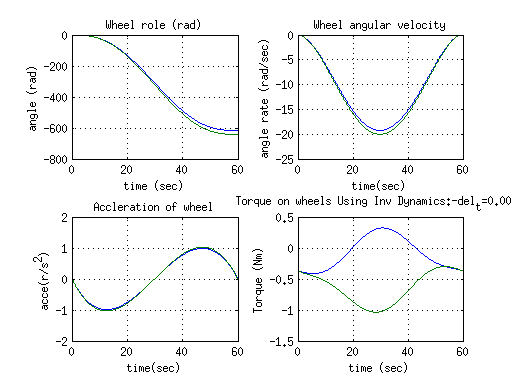
\includegraphics[height=300pt,keepaspectratio]{Chapter4/fig/FD}
	\captionof{figure}{Inverse Dynamics of Mobile Robot moving up on $15^o$ ramp }
	\label{fig:spiral} 
\end{figure} 
%
\begin{table}[!htbp]
	\caption{Dynamic parameters used in forward dynamic simulation.}
	\label{tb:massproperty}
	\centering
	\begin{tabular}{l l l}
		\hline
		\emph{Part Name}  & \emph{Mass Property} & \emph{Value} \\
		\hline
		Rear Wheels  & mass &300g \\ 
		 & Moment of Inertia & diag(242, 242, 465)kg $mm^2$\\
		Base Frame & mass & 70Kg \\
		 & Moment Of Inertia & $ \begin{pmatrix}
		 1.18& 0.01&-0.05\\ 0.01 & 1.28 & 0.08\\
		 -0.05 & 0.08 & 0.53
		 \end{pmatrix} Kg-m^2$ \\
		\hline
	\end{tabular}
\end{table}
 
\section{Conclusion}
We have presented the dynamic equation of the most general form of caster wheel configuration. Even though we have considered here only two caster wheel the formulation can be extended to any number of caster wheels, in such case we have to find equation \ref{unac2act1} for each caster wheel system, and then proceed mechanical as to calculate the corresponding twists. We have also shown that the  dynamic of standard caster wheels is a special case of our general case with $d_1=0$. We have also proved why a caster needs a non-zero caster offset distance, and the  need of extra actuators in case $d_2=0$.
    



\section{Summary}
In this chapter, 

